Our work closes the loop in VQS sensemaking so that VQS works in scenarios  where XY is unknown or Z is unknown. These areas were previously unexplored by past works.
%%%%%%%%%%%%%%%%%%%%%%%%%%%%%%%%%%%%%%%%%%%%%%%%
\begin{figure}[h!]
  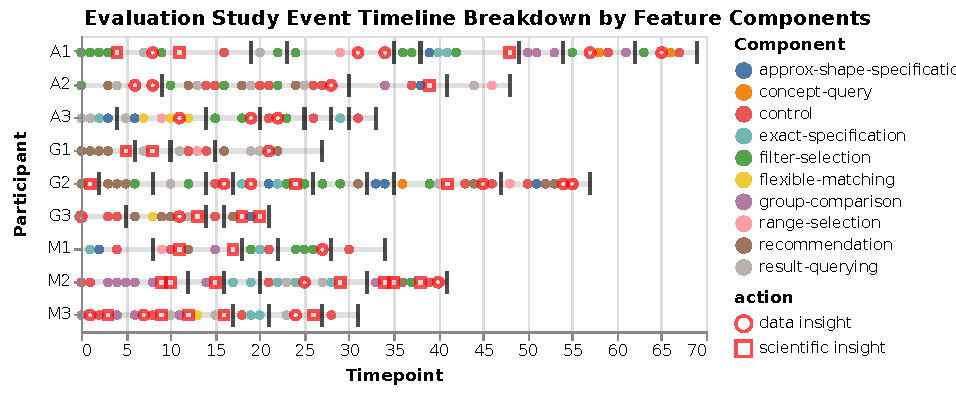
\includegraphics[width=\linewidth]{figures/evalstudytimeline.pdf}
  \caption{Timeline of event code and component usage, with every timepoint as an event on the x axis. For clarity, we hide most of the event coding labels other than the insight labels. Black vertical tick indicates a session break, signaling the beginning of a new line of inquiry.}\label{fig:evalstudytimeline}
\end{figure}
In Figure~\ref{fig:evalstudytimeline}, we map the features to components based on the taxonomy described in Figure~\ref{fig:taxonomy} to plot the timeline of event codes and component usage for each participant.
%%%%%%%%%%%%%%%%%%%%%%%%%%%%%%%%%%%%%%%%%%%%%%%%
\par The three paradigm that we have described are not mutually exclusive categories. In fact, we find that participants often construct a central workflow focused on features from one of the main paradigms and interleave variations with the feature usage from the two other paradigms as they iterate on the analytic task, as shown in Figure~\ref{fig:usagefreqbysubject}. As we have seen, the central paradigm adopted by each use case is tightly coupled with characteristics of the analytic challenges presented by the use cases. Next, we will describe some of the design principles (DP) based on our study findings.
\begin{figure}[h!]
  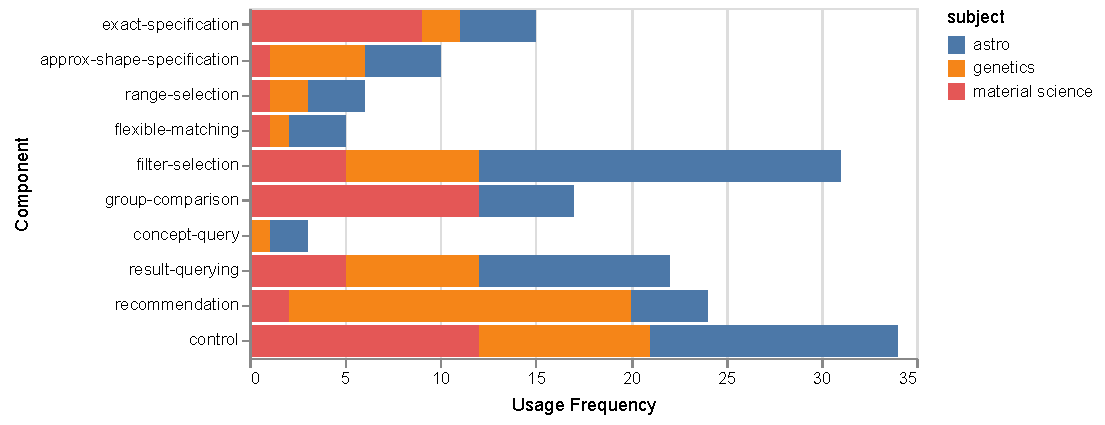
\includegraphics[width=\linewidth]{figures/usagefreqbysubject.pdf}
  \caption{The number of times each component is used during the evaluation study, broken down by subject areas. Astronomers largely focused on filtering, whereas material scientists made heavy use of dynamic class and geneticists made use of recommendations heavily.}\label{fig:usagefreqbysubject}
\end{figure}
